\chapter{Dataset e Competizioni}

Nonostante negli anni nel mondo della Computer Vision vi sia sempre stata una necessità di dataset pubblici per la comparazione di metodi concorrenti, i dati a disposizione su cui lavorare sono stati invece relativamente esigui poiché la gran parte dei problemi venivano solitamente risolti con un approccio di tipo analitico.\par
Da quando però nell'ultima decade è avvenuto un cambiamento nel modo di porsi a molte sfide grazie all'adozione delle reti neurali come strumento per l'apprendimento automatico, questa esigenza, aiutata anche dell'arrivo dei cosiddetti \textit{Big Data}, si è espansa in svariati settori dell'informatica.\par 
Il bisogno sempre più crescente di dati, nella nostra area di interesse di tipo visivo, però non è esente da problematiche: per l'apprendimento automatico sono infatti richiesti dati costituenti una \textit{groundtruth}, ovvero informazioni che rappresentino verosimilmente la soluzione del problema postosi, e perciò non generabili in gran quantità ed automaticamente da un elaboratore.\par
Dataset degni di nota nel campo della Computer Vision che si sono imposti come standard nell'ambito dell'\textit{object detection} sono il PASCAL Visual Object Classes~\cite{pascalvoc}, ImageNet~\cite{imagenet} ed il più recente MSCOCO~\cite{mscoco}.\par
Di seguito approfondiremo i vari dataset a nostra disposizione per il task della localizzazione del testo e i principali metodi di valutazione proposti nella letteratura e adottati da varie competizioni.

\section{Dataset}

\subsection{Focused Scene Text}
\label{subsec:focused}
Introdotto per la prima volta in occasione di ICDAR2013~\cite{ICDAR2013}, è composto da immagini acquisite in contesti reali dove l'oggetto principale è un'area di testo, solitamente orizzontale e formata da caratteri alfanumerici.\\
Nasce quindi avendo in mente i casi d'uso più comuni, quali la lettura del testo ed eventualmente una sua traduzione, portando dunque in secondo piano la fase di localizzazione, resa più immediata, a favore di un focus sulla precisa segmentazione e riconoscimento delle singole parole e/o lettere.\par
Caratteristiche:
\begin{itemize}
	\item
		229 immagini di training
	\item
		233 immagini di test
	\item
		groundtruth composta dalle coordinate delle bounding box ortogonali e trascrizione di ogni singola parola
\end{itemize}

\subsection{Incidental Scene Text}
\label{subsec:incidental}
Introdotto per la prima volta nell'omonima competizione in occasione della conferenza ICDAR2015~\cite{ICDAR2015}, è composto da immagini acquisite in contesti reali (attraverso fotocamere indossabili) dove le aree di testo non sono l'oggetto principale e possono dunque trovarsi a diverse distanze e posizioni.\\
Questa differenza con il dataset precedente lo rende più adatto come metro di valutazione per il task su cui ci concentreremo in questa tesi in quanto la fase di localizzazione viene resa meno triviale. Verrà usato anche per la comparazione con metodi concorrenti.\par
Caratteristiche:
\begin{itemize}
	\item
		$1000$ immagini di training
	\item
		$500$ immagini di test
	\item
		groundtruth composta dalle coordinate dei vertici delle bounding box orientate e trascrizione di ogni singola parola (quando leggibile)
\end{itemize}


\begin{figure}[H]
	\centering
	\begin{subfigure}[b]{0.4\textwidth}
		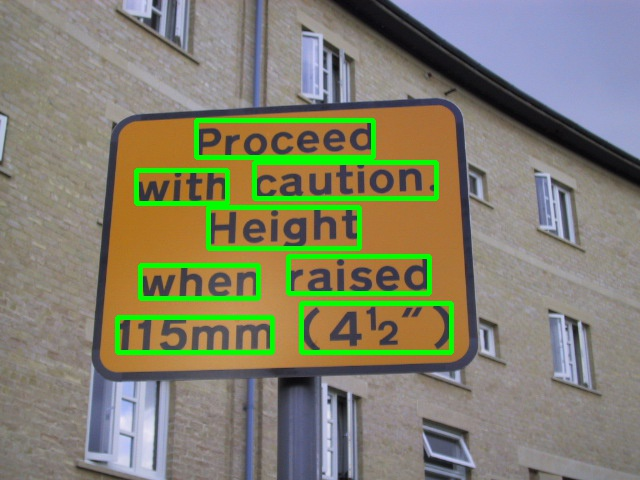
\includegraphics[width=\textwidth,trim={2cm 0 4cm 0},clip]{focused_example.jpg}
		\caption{Focused Text Scene}
	\end{subfigure}
	\hfill
	\begin{subfigure}[b]{0.55\textwidth}
		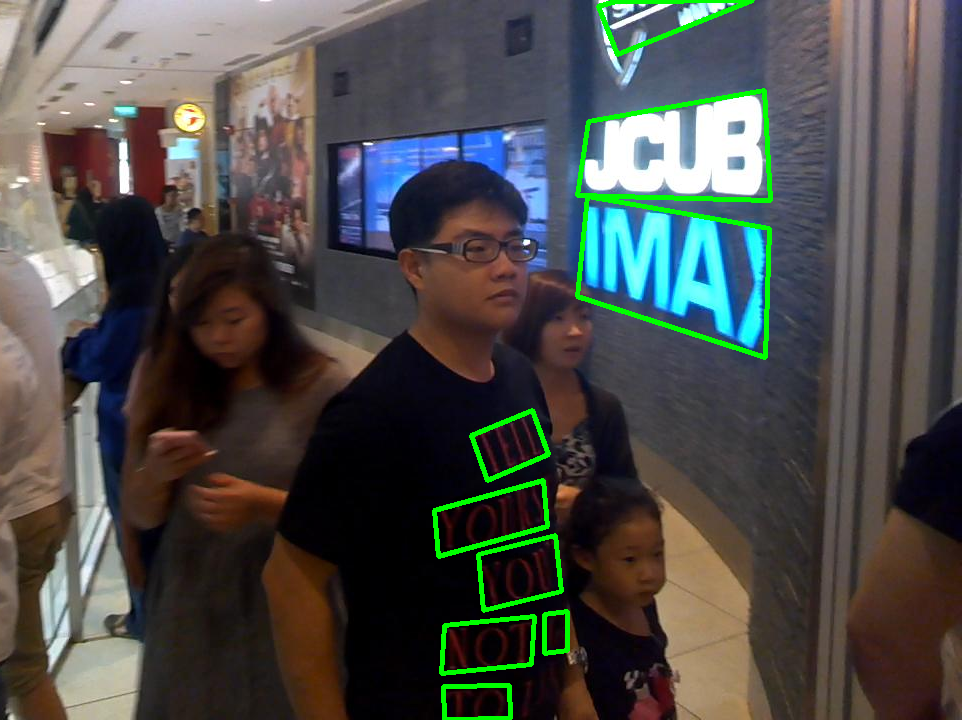
\includegraphics[width=\textwidth]{incidental_example.png}
		\caption{Incidental Text Scene.}
	\end{subfigure}
	\caption{Immagini di training con relative annotazioni.}
	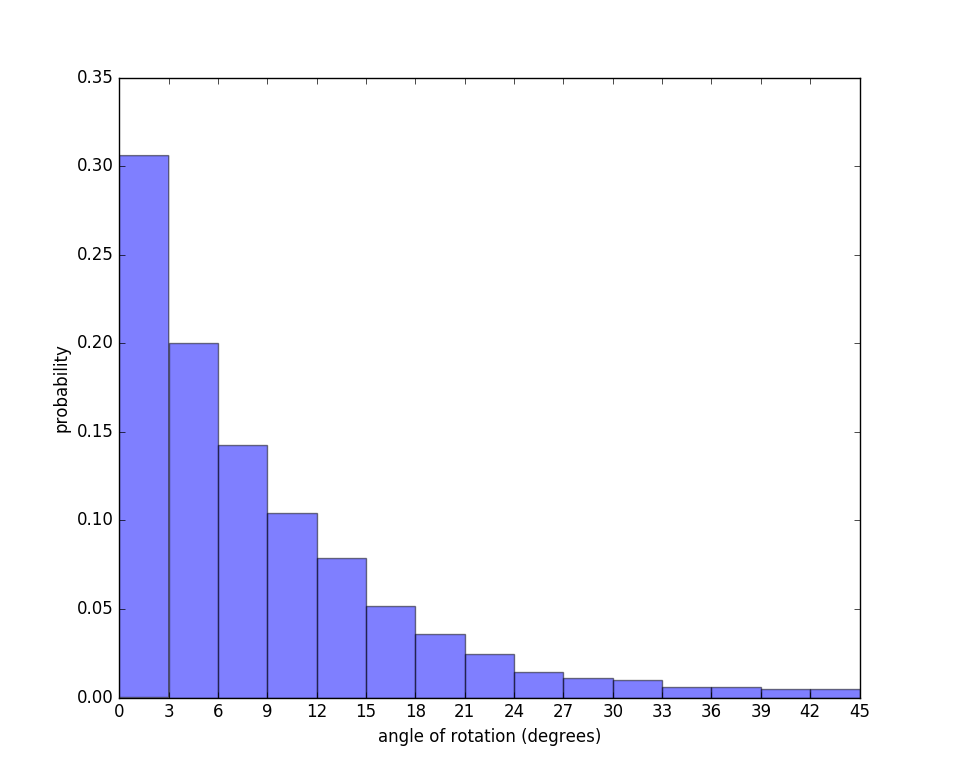
\includegraphics[width=\textwidth]{incidental_rotation.png}
	\caption{Angoli di rotazione delle bounding box in Incidental Text Scene.}
\end{figure}

\subsection{COCO Text}
\label{subsec:coco}
Introdotto nel 2016~\cite{cocotext} come estensione del MSCOCO Dataset, viene in seguito utilizzato per l'omonima competizione in occasione di ICDAR2017.
Punti di forza di questo dataset, oltre alla grande quantità di immagini, sono la varietà di contesti di acquisizione e la eterogeneità delle classi delle annotazioni. Per questo motivo lo si è scelto come base di training per i nostri esperimenti e come base per la validazione delle performance.\\
Non ci è possibile confrontarci con metodi concorrenti in quanto i risultati della competizione non sono ancora stati resi pubblici.\par
Caratteristiche:
\begin{itemize}
	\item
		$43.686$ immagini di training (118.309 parole)
	\item
		$10.000$ immagini di validation (27.550 parole)
	\item
		$10.000$ immagini di test
	\item
		groundtruth composta da bounding box ortogonali e trascrizione per ogni parola, ognuna con i seguenti attributi:
		\begin{itemize}
			\item
				machine printed / handwritten / altro
			\item
				leggibile / illeggibile
			\item
				inglese / non-inglese / sconosciuto
		\end{itemize}
\end{itemize}

\begin{figure}[H]
	\centering
	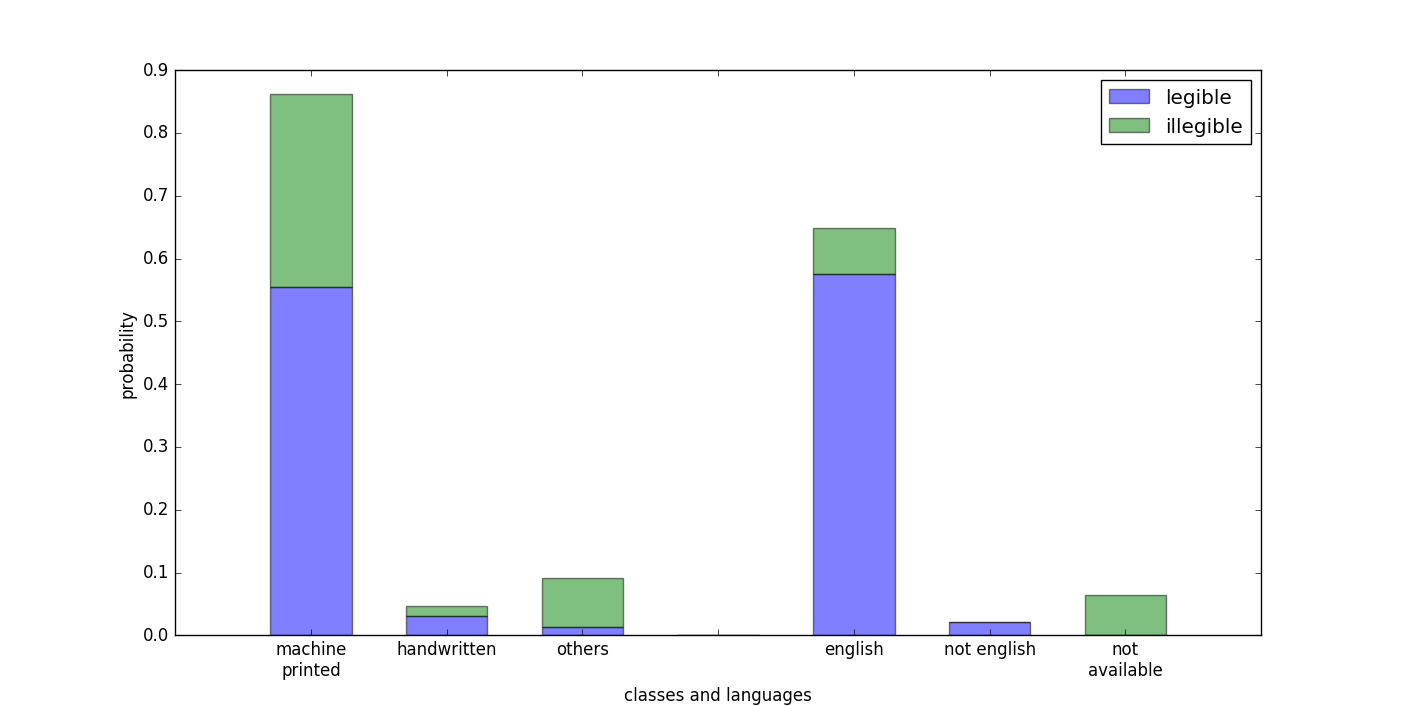
\includegraphics[width=1\textwidth]{annotation_classes_languages.png}
	\caption{Classificazione delle annotazioni}
\end{figure}

\subsection{SynthText}
\label{subsec:synth}
Introdotto nel 2016~\cite{synthtext}, ma mai utilizzato come base di training in nessuna competizione, la peculiarità di questo dataset risiede nel fatto che il testo è inserito sinteticamente, con una certa context-awareness, in immagini reali.\par
Caratteristiche:
\begin{itemize}
	\item
		$858.750$ immagini
	\item
		$7.266.866$ parole
	\item
		$28.971.487$ lettere
	\item
		groundtruth composta da trascrizioni e coordinate dei vertici delle bounding box orientate di ogni parola ed ogni singola lettera
\end{itemize}
\vfill
\begin{figure}[H]
	\centering
	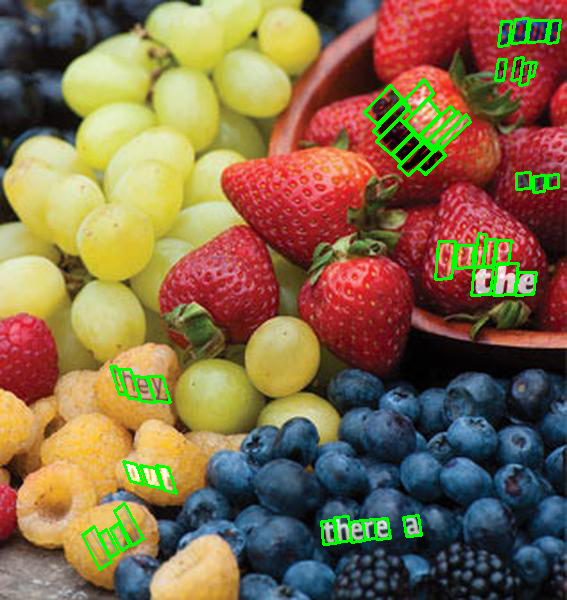
\includegraphics[width=0.7\textwidth]{synth_example.png}
	\caption{Immagine di training SynthText}
\end{figure}

\begin{figure}[H]
	\centering
	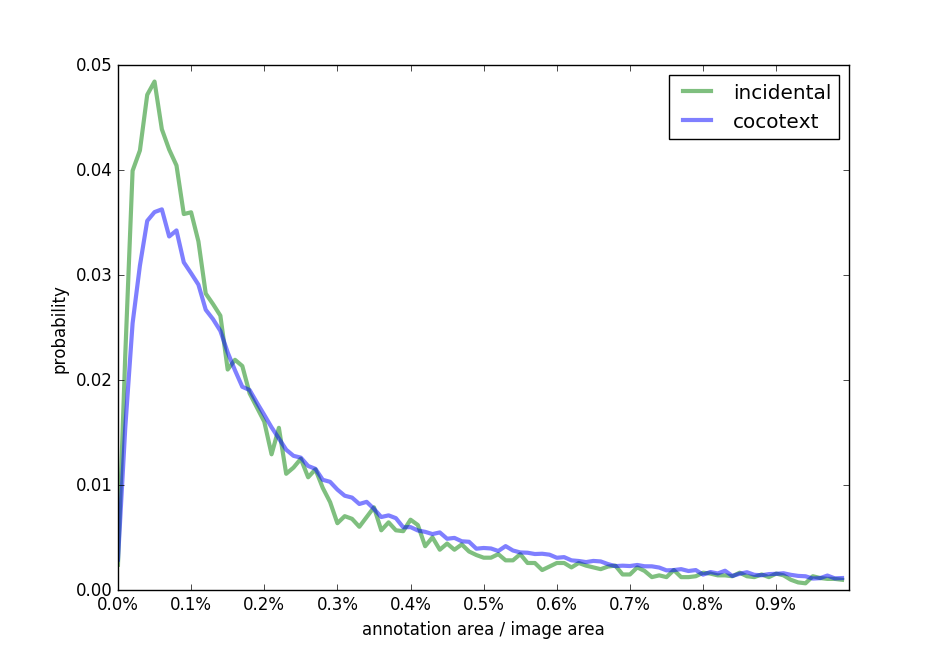
\includegraphics[width=\textwidth]{annotation_ratio.png}
	\caption{Area occupata dalle singole annotazioni nalle rispettive immagini}\label{fig:annratio}
	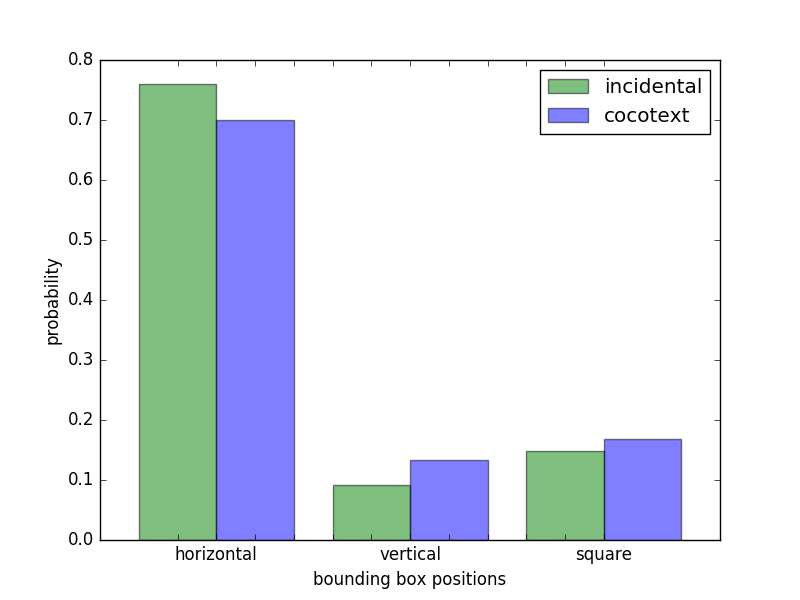
\includegraphics[width=0.9\textwidth]{annotation_position.png}
	\caption{Proporzioni delle upright bounding box}\label{fig:annprop}
\end{figure}



\section{Metodi di valutazione}
Come già precedentemente annoverato, per la comparazione tra metodi diversi che concorrono per lo stesso fine, si necessita di valori di riferimento omogenei e significativi.
In seguito verranno dunque illustrati più in dettaglio i vari metri di valutazione presenti in letteratura utilizzati per i nostri esperimenti e competizioni di riferimento.\par

\subsection{Precision \& Recall}
Quelle che seguono in questa sezione sono statistiche generali per la classificazione binaria indipendenti dallo specifico task.

\subsubsection{Precision}
Indica la percentuale di predizioni corrette rispetto al numero di predizioni totali.
Viene calcolata come segue:
$$
\text{precision} = \frac{\text{true positives}}{\text{true positives} + \text{false positives}} = \frac{tp}{n}
$$

\subsubsection{Recall}
Indica la percentuale di predizioni corrette rispetto al numero di istanze significative totali.
Viene calcolata come segue:
$$
\text{recall} = \frac{\text{true positives}}{\text{true positives} + \text{false negatives}}
$$

\subsubsection{F1-score}
Questa misura prende in considerazione entrambi i criteri precedentemente descritti calcolandone la media armonica, evitando perciò i problemi che potrebbero nascere dalla semplice media artimetica qualora la recall fosse molto bassa e la precision alta (poche predizioni ma corrette) e viceversa (molte predizioni fra cui molte erronee).
$$
F_{1} =
		\frac{2}{\frac{1}{\text{recall}} + \frac{1}{\text{precision}}}
	  =
		2 \cdot \frac{\text{precision} \cdot {\text{recall}}}{\text{precision} + \text{recall}}
$$

\subsubsection{Average Precision}
Anche questa stima utilizza sia la precision che la recall, ma in più necessita di un livello di confidenza per ogni predizione in modo da poter calcolare una curva di precision/recall dalla qualle estrarre l'area sottostante, il cui valore corrisponde alla precisione media. Quantizzata risulta calcolabile come:
$$
\sum_{k=1}^{N}{P(k) \Delta r(k)}
$$
dove $N$ è il numero totale di predizioni, $P(k)$ è la precisione al livello di confidenza $k$ e $\Delta r(k)$ è la differenza tra i valori di recall tra gli step di confidenza $k-1$ e $k$.

\subsection{Intersection over Union}
Se prima abbiamo visto metri di valutazione generici, quello qui descritto è invece specifico del campo dell'object detection.
Infatti poiché nei task di rilevamento risulta altamente improbabile predire un match esatto di una bounding box, è nata la necessità di uno standard di valutazione coerente ed efficace con il quale si potesse distinguire un \textit{vero positivo} da un \textit{falso positivo} influenzando di conseguenza tutte le misure descritte fin'ora.\par
Come suggerito dal nome, questa metrica è calcolata prendendo il rapporto tra l'area dell'intersezione e l'area dell'unione di due bounding box, predizione e groundtruth. Essendo il risultato un semplice valore numerico, è necessario porre una soglia per l'avvenuta detection, solitamente impostata a $0.5$ (oppure $0.75$ per valutazioni più meticolose).\par
Una delle caratteristiche principali dell'IoU è la penalizzazione dei casi in cui oggetti multipli appartenenti alla stessa classe vengano rilevati in una bounding box unica, ma specularmente si rischia di avere risultati ingannevoli nel caso in cui le annotazioni presentino errori o qualora il modello riesca addirittura a superare l'accuretezza della groundtruth.\par

\begin{figure}[H]
	\centering
	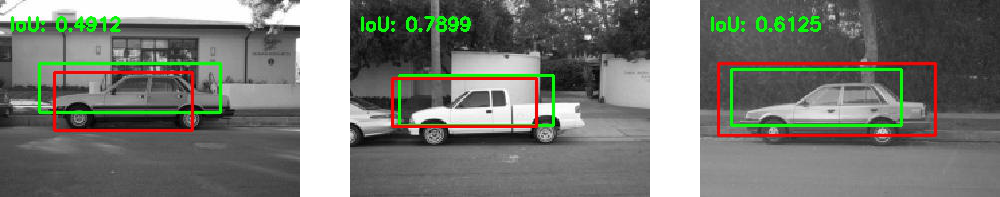
\includegraphics[width=\textwidth]{iou.png}
	\caption{Esempi di valutazione con IoU.}
\end{figure}

